\chapter{The case of tokamak devices}
\label{ch:tokamaks}
\doublespacing
\vspace{-2.5cm}

The previous chapter motivated the importance of the proposed DUA framework and of the technologies on which it is based in the context of autonomous robots. It clarified the relevance of the proposed solution in that context and provided some preliminary results that suggest its potential, as well as some practical application that benefited of the DUA structure. This chapter focuses on a different, yet related context: that of tokamak devices for nuclear fusion with magnetic plasma confinement.

From the point of view of a system architecture developer, these two scenarios are not so different: both involve complex systems with many interacting components and both require a high degree of autonomy. However, autonomy is the first item that differentiates these contexts: an autonomous robot, as discussed in \Cref{ch:prb,ch:robots}, is a single entity that may have to operate independently for long periods of time, while a tokamak device may even surpass a robot in terms of complexity but it is an experimental device; this implies that it is not expected to operate without human operators involved and that its operational times might be shorter than those of a robot. Nonetheless, the various subsystems of a tokamak device are usually expected to operate autonomously during an experiment, thus the technologies and design paradigms discussed previously are still relevant. Among those, as the following clarifies, the distributed paradigm remains among the most suitable since the control system of a tokamak may be made of a variety of components that need to communicate and coordinate with each other.

Tokamak device are another application scenario for the work developed for this thesis. This chapter presents the concepts of nuclear fusion with magnetic confinement and plasma shape control, then introduces the Tokamak à Configuration Variable (TCV) device that has been the subject of this work. Subsequently, two innovations are presented: an application of the distributed DDS middleware (see \Cref{sec:dds}) to the TCV control architecture, and the dynamic optimization of the coil currents for plasma shape control, both made possible by the versatility of TCV's distributed control system.

\section{An introduction to magnetic confinement fusion}
\label{sec:tokamaks_intro}

Nuclear fusion occurs when light atomic nuclei combine to form heavier elements. This process powers stellar bodies and represents a promising avenue for clean, sustainable energy generation. These reactions, such as the fusion of Deuterium and Tritium nuclei to produce an $\alpha$-particle and a high-energy neutron, release substantial energy with the potential for efficient power generation.

The development of fusion energy has acquired heightened significance in the context of contemporary global challenges. As nations worldwide confront climate change and seek to reduce greenhouse gas emissions, fusion technology offers a carbon-neutral alternative to fossil fuels. Furthermore, fusion power could address the growing energy demands of emerging economies while promoting sustainable development, as it requires minimal fuel resources and produces no long-lived radioactive waste like fission does. The abundance of fusion fuel sources in nature also promises enhanced energy security and reduced geopolitical tensions associated with conventional energy resources. Moreover, nuclear power plants can be scaled to meet the demand of the territory in which they are located, without the need to identify suitable locations to harvest renewable but intrinsically intermitted sources of energy such as solar or wind.

To facilitate fusion reactions, the participating elements must be heated to temperatures sufficient for charged nuclei to overcome their repulsive Coulomb forces. At these elevated temperatures, the matter exists as fully ionized gas, termed \emph{plasma} \cite{chen_introduction_2012}, which must be confined for durations adequate to achieve practical reaction probabilities.

Tokamaks \cite{wesson_tokamaks_2011} are experimental devices that have originated in the 1950s in the USSR; \Cref{fig:tcv_schematic} depicts the TCV machine, which has been the subject of this work. They employ toroidal vacuum chambers for plasma confinement using magnetic field configurations \cite{ariola_magnetic_2008,braams_nuclear_2002,esposito_runaway_2016}. Dedicated coils encircling the chamber generate a \emph{toroidal} magnetic field, while \emph{poloidal} field coils produce an \emph{axisymmetric} poloidal field. This poloidal field serves multiple functions: controlling plasma position and shape while inducing \emph{plasma current}; the plasma must, in fact, carry a current that is instrumental to keep the fusion reaction going, as well as to maintain a reference temperature. Over the decades, tokamaks have contributed to study the behavior of plasma among different types of reactions, as well as to develop the technologies necessary to improve and maintain magnetic confinement. More recent devices, such as the ITER and the JT-60SA machines, incorporate the generation of energy into their project goals.
\begin{figure}[t!]
  \centering
  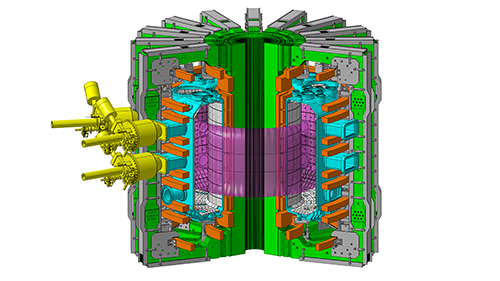
\includegraphics[width=.8\textwidth]{images/ch6/tcv_schematic.jpg}
  \caption{Schematic of the TCV device.}
  \label{fig:tcv_schematic}
\end{figure}

Plasma configurations, characterized by distinct cross-sectional geometries in the poloidal plane, exhibit varying properties regarding stability, performance, and interaction with vessel components. The plasma shape significantly influences the stability characteristics of global \emph{magnetohydrodynamic} (MHD) modes and regulates particle transport phenomena. Furthermore, precise plasma shaping enables optimization of chamber utilization and plasma volume while facilitating controlled management of power deposition from plasma-wall interactions in regions where energy escapes the confined plasma core. To define a plasma shape and its position, two key elements are considered: the \emph{centroid} and the \emph{last closed flux surface} (LCFS).

The centroid is the center of the plasma cross-section along the poloidal plane, and can be either \emph{magnetic} or \emph{geometric}; the type of centroid to consider depends on the specific application at hand. The magnetic centroid is usually involved when it is convenient to approximate the plasma as a filament carrying the plasma current; in that case, the magnetic centroid corresponds to this ideal filament revolving around the vessel. The geometric centroid, on the other hand, can be considered when no such approximation is relevant and the entirety of the plasma cross-section within the vessel must be taken into account. When dealing with magnetic control, which is also the case of this work, the magnetic centroid is usually considered.

Poloidal field coils, running along the torus, generate a poloidal field that induces a \emph{poloidal flux} in the vessel. Along the plasma volume, there are points in which this flux has the same value. Examining the plasma from a poloidal cross-section, one can group this points by flux values, thus identifying \emph{isoflux surfaces}. These run outward starting from the plasma centroid, initially as closed surfaces that enclose one another. The last closed one of these surfaces is identified as the LCFS.

Thus, controlling the plasma shape usually involves tracking reference setpoints for the centroid and the LCFS, expressed as a set of control points \cite{mele_design_2024,tenaglia_unified_2024}. The shape control capabilities directly impact operational parameters and plasma-material interactions, allowing for advanced scenarios that maximize performance while preserving machine integrity. This type of control represents a critical tool for achieving optimal plasma conditions while maintaining operational safety margins. To achieve different plasma configurations in terms of shape, the machine must be equipped with both a vessel large enough to contain them and with a set of coils that can generate the necessary magnetic fields.

The control infrastructure of a tokamak fusion device represents a sophisticated integration of diverse technological components operating across multiple temporal and spatial scales. The hardware architecture encompasses an extensive array of elements: high-power electrical supplies for magnetic field generation, Programmable Logic Controllers (PLCs) for real-time control and safety systems, analog control and diagnostic devices, and server-grade computing systems for data acquisition and processing. This hardware foundation must support both high-bandwidth real-time operations and complex experimental procedures while maintaining strict safety protocols.

The operational complexity extends beyond hardware considerations to include intricate control schemes for plasma magnetic confinement, comprehensive diagnostic systems for plasma state monitoring, and experimental execution frameworks. These systems must operate in concert to maintain plasma stability while facilitating scientific investigation. The human interface component adds another layer of complexity, requiring control rooms staffed by teams of skilled operators managing different aspects of machine operation. The supervision infrastructure must provide interfaces ranging from detailed module-level control to high-level Supervisory Control and Data Acquisition (SCADA) systems, enabling both fine-grained control and system-wide monitoring.

Such operational sophistication demands a robust and well-structured architectural foundation. The control system design must accommodate real-time requirements, ensure fault tolerance, and facilitate system maintenance and upgrades. A distributed systems paradigm offers particularly compelling advantages in this context, providing natural solutions for parallel operation, redundancy, and scalability. This approach enables effective management of the inherent complexity of the system while maintaining the flexibility necessary for experimental physics operations.

\subsection{The Tokamak à Configuration Variable}
\label{sec:tcv}
There are various dimensional parameters that can be used to evaluate the size of a tokamak device; one of these is the \emph{major radius} $R_0$, which is the distance from the center of the torus to the outer wall of the vessel. With a major radius $R_0=\SI{0.88}{\meter}$, TCV is classified as a medium-scale fusion research device. It is operated at the Swiss Plasma Center (SPC) of the École Polytechnique Fédérale de Lausanne (EPFL), Switzerland \cite{lister_control_1997}. The device designation reflects its exceptional plasma shaping capabilities, enabled by an extensive array of independent Poloidal Field (PF) coils in conjunction with a distinctive rectangular vacuum vessel geometry, achieving toroidal magnetic fields up to \SI{1.54}{\tesla}.

The PF coil system, illustrated in \Cref{fig:tcv_layout}, comprises four distinct subsystems.
\begin{itemize}
  \item The \textbf{OH coils}, consisting of a central solenoid (OH1) and an up-down symmetric arrangement of 6 series-connected coils (OH2), provide plasma current drive functionality.
  \item The \textbf{E coils}, comprising 8 independently controlled circuits positioned on the high-field side.
  \item The \textbf{F coils}, featuring 8 independent circuits located on the low-field side.
  \item The \textbf{G coils}, consisting of two up-down symmetric in-vessel coils in anti-series configuration for vertical stabilization of the plasma.
\end{itemize}
The device architecture accommodates removable \emph{baffles} \cite{reimerdes_initial_2021} that enhance plasma core-divertor separation. The configuration depicted in \Cref{fig:tcv_layout} shows the Short-Inner-Long-Outer (SI-LO) baffles arrangement.
\begin{figure}[t!]
  \centering
  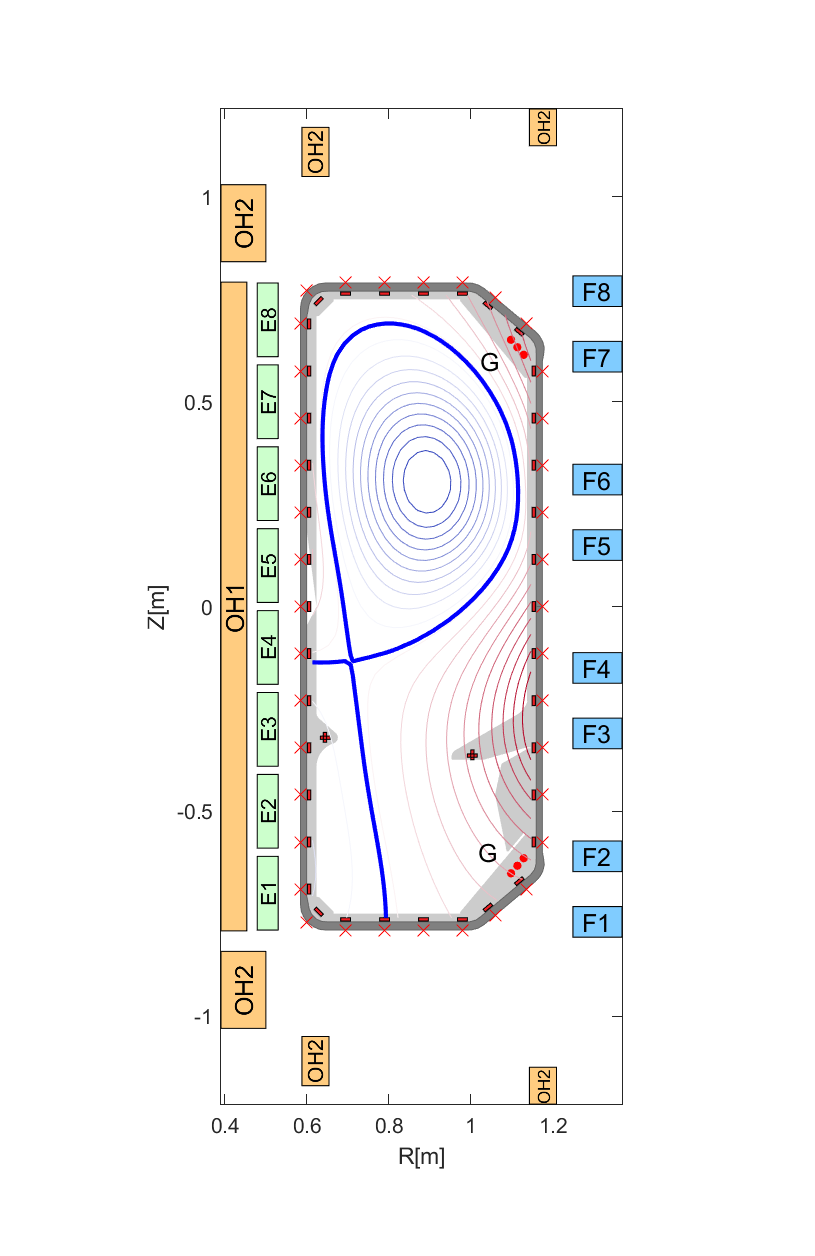
\includegraphics[scale=.6]{images/ch6/tcv_layout.eps}
  \caption{TCV poloidal cross-section with an example plasma configuration (lower single-null). The OH, E, F, and G coils are highlighted in different yellow, green, blue, and red, respectively. Removable baffles appear in the cross-section in gray protruding inward in the bottom part of the vessel.}
  \label{fig:tcv_layout}
\end{figure}

The exceptional plasma shaping capabilities of TCV, combined with its continuously enhanced control architecture, have established this device as a significant contributor to international fusion research \cite{duval_experimental_2024}. Through successive upgrades to both hardware and control systems spanning its three decades of operation, TCV has maintained its position at the forefront of experimental fusion science. Its contributions span multiple international research campaigns \cite{joffrin_overview_2024}, including investigations of advanced plasma configurations and real-time control developments.

\section{Improving the SCD network with the DDS}
\label{sec:ddstcv}
The strict real-time requirements of a sophisticated control system such as the SCD, described in \Cref{sec:scd}, ask for an implementation that is designed and configured for the task at hand in any of its parts. Operating system kernels must be compiled with patches that enable fine-grained real-time task scheduling policies. The software must be written with frameworks that guarantee real-time execution, such as MARTe2. The hardware must be powerful enough to handle the computational load of the control algorithms, reserving to them all the system resources they require (\emph{e.g.}, CPU, RAM, PCI bandwidth) in a deterministic fashion, cutting out every other task including system ones. When sampling times get to the microsecond precision declared in \Cref{sec:scd}, every component of the system must be carefully considered.

In this scenario, things are a bit complicated by the fact that SCD is \emph{distributed} in the sense that has been described in \Cref{ch:intro}. It is not a single system but an interconnection of multiple computational nodes each executing a predefined set of tasks encoded in specific software subsystem, also interfacing with dedicated hardware components when necessary. Each node cannot perform its tasks alone: for example, control nodes 02 and 03 cannot actuate the coil power supplies properly without the real-time data provided by the plasma equilibrium reconstruction, which runs on nodes 05 and 06, which in turn need the data from the plasma diagnostics running on other nodes. By this description, it is clear how the communication infrastructure among the nodes must be carefully designed and implemented to guarantee the real-time performance of the whole system. It must employ a technology that makes it fast, deterministic, and reliable.

Currently (see \cite{galperti_overview_2024}), the SCD nodes are interconnected by a real-time fiber optic network that implements a \emph{reflective memory} (RFM). In essence, reflective memories are shared memory systems that allow multiple machines to share a data area. The implementation of the RFM usually consists of a high-speed connection medium, in this case an optic fiber connection, and dedicated network cards to install on the machines forming the network. These cards contain the actual data area, and their device drivers map that area within the main memory of the host machine. The RFM implementation is such that each local copy of the shared data area is kept coherent with the others, so that every write operation is propagated to all the other copies. The timings that these operations might take can be very tight but, most importantly, they are deterministic. This makes the RFM a suitable technology for this kind of application scenario.

The RFM technology has been commercially available since the 1980s and SCD adopts Abaco Systems network cards \cite{abaco_systems_pcie-5565rc_nodate}. As stated in \Cref{sec:scd}, these cards and their fiber optic interconnection allow SCD to maintain sub-microsecond latencies when transferring data among the nodes with a throughput up to \SI{170}{\mega\byte/\second}. This implementation has allowed SCD to perform well in the last decade but it is now showing some concerning issues, especially in terms of scalability and maintainability. First, as stated in \cite{abaco_systems_pcie-5565rc_nodate}, the Abaco cards are reaching their End Of Life (EOL) status with a limited production phase started in 2022. This, together with their high price (around 8.000€/card), is creating procurement concerns at SPC for such a critical component of the SCD. Secondly, the throughput of the RFM network is not enough to handle the increasing amount of data that the SCD nodes must exchange. New diagnostics are being evaluated and added each year, with some of them capable of generating considerable amounts of data, such as the MANTIS camera system on Node 10. The problem becomes clear when one notes that the data area is shared among \emph{all} the nodes, so they have to use that space to exchange data coming from every device and subsystem all at the same time. Despite some access policies that have been implemented to deal with this without increasing latencies (see, again, \cite{galperti_overview_2024}), a saturation point has been reached and new diagnostics such as bolometry cannot currently be used in real-time control because their data cannot be shared among the nodes.

To allow further upgrades to the SCD increasing TCV's experimental capabilities, as well as to avoid ending up relying on an EOL component, a replacement solutions for the RFM network has become necessary. Various criteria have been applied to its selection, including the cost-effectiveness of relying again on dedicated hardware components when common network hardware such as Ethernet has evolved so much in the meantime, guaranteeing bandwidths that were simply unthinkable at the time in which the reflective memory was invented. Ideally, a properly configured, reserved Ethernet network is enough if it driven by a software protocol that is able to guarantee the same determinism and low latencies of the RFM. The Data Distribution Service, introduced in \Cref{sec:dds}, is a candidate technology that can provide these features and has been selected as a replacement for the RFM network in the SCD.

This section describes the design of a software component for the SCD architecture that integrates the DDS middleware for communication purposes. Then, it presents some preliminary results of its application on SCD nodes, showing promising performance that motivated the decision to proceed with the integration of the DDS in the SCD. These results prove how the distributed technologies that constitute the base of the DUA framework presented in \Cref{ch:dua} can be applied successfully even to a different context such as the control system of a tokamak device.

\section{Dynamic control allocation for plasma shape control}
\label{sec:allocation}
In \Cref{sec:tokamaks_intro}, the second application scenario of this work has been introduced. In particular, \Cref{sec:tcv} illustrated the Tokamak à Configuration Variable device, and \Cref{sec:scd} corroborated it with a thorough description of the Système de Contrôle Distribué that controls TCV. That description clarified how the distributed control system of TCV allows multiple diagnostics, algorithms, estimators, and controller to coexist and interact within a single control architecture. Thanks to this design, the experimental capabilities of TCV have been extended since the days of the original implementation of the SCD. One of the latest innovations in this context has been the introduction of a \emph{shape controller} \cite{mele_design_2024}, \emph{i.e.}, a subsystem that acts as a reference governor and PID controller for the coil power supplies in order to track a desired plasma shape. Its implementation currently works in coordination with other SCD subsystem, in particular those that generate feedback measurements concerning the equilibrium reconstruction, that are used to evaluate the control law in real-time.

Even if the current design of the TCV shape controller might seem simple, it has been quite the challenge for the development team, and its integration and tuning have turned out to be quite delicate tasks. The end result is a system that works: given a reference plasma shape and after some tuning, it is able to control the plasma shape within the limits of the actuators and the diagnostics. Recalling what has been said in \Cref{sec:tcv}, \emph{i.e.}, the discussion of the redundant coil configuration that constitutes probably the most peculiar feature of TCV itself, one question arises: how does the shape controller take advantage of this redundancy to improve the performance of the coil current control? Up to this stage, it does not. The PID formulation of the shape controller, thoroughly described in \cite{mele_design_2024}, does not account for the actuator redundancy offered by the TCV model, which could in turn be exploited to improve the performance of the shape controller itself. Performance indicators to be considered in this context are the tracking error of the plasma shape, as well as the overall power consumption of the coils or even the saturation limits of the power supplies. In practical experiments, these have turned out to be quite important aspects to consider when working on TCV.

The aforementioned question is the starting point for the work presented in this section, which concerns a specific subject of control theory that is receiving increasing interest in recent years: that of dynamic control allocation. Techniques belonging to this subject are used to distribute the control effort among a set of redundant actuators in order to optimize a given performance index, thus following an \emph{allocation policy}. What distinguishes \emph{dynamic} control allocation from similar techniques is that, in the former, the allocation policy is a control law itself that is determined through a control design process and evaluated in real-time. Subsystems that are typically involved in a dynamic control allocation scheme are denoted as \emph{dynamic allocators} or simply as \emph{allocators}. The peculiarity of dynamic allocators is that they are designed as \emph{add-ons} to a preexisting control system, \emph{i.e.}, their design does not require a complete redesign of the control system, which could yield significant complications when optimization objectives are included in the problem. Instead, given the models of the plant and the control system, their design can be carried out \emph{a posteriori}, and then they can be integrated into the control system as additional components properly connected to the control loop. The art of dynamic control allocation, therefore, lies in the design of these additional components with the goal in mind of not only optimizing the control action in terms of some criteria of practical relevance, but also of ensuring that the original control objectives are still met, possibly without any alteration of the desired output behavior.

Regarding TCV, a preliminary study has been carried out in \cite{tenaglia_dynamic_2024}, in which an early implementation of a dynamic coil current allocator has been integrated in the MATLAB code suite of TCV. Its performance has been validated by means of simulations on real shot data, which showed the feasibility of this approach. This section presents the work that has been carried out in this direction. First, a review of the current state of the art about dynamic control allocation is presented, together with a set of formulations that are of interest for the TCV case. Each of these has been considered, leading to some independent theoretical results that are reported in the following. Then, the design of a novel dynamic control allocator for TCV is presented, which is based on the latest advancements on the subject. At the end of the section, experimental results are discussed, which show the performance of the proposed novel allocator in a real scenario and constitute the first working implementation of its kind in the literature.

